\documentclass[10pt,xcolor=pdflatex]{beamer}
\usepackage{newcent}
\usepackage[utf8]{inputenc}
\usepackage[slovak]{babel}
\usepackage{hyperref}
\usepackage{fancyvrb}
\usetheme{FIT}

%%%%%%%%%%%%%%%%%%%%%%%%%%%%%%%%%%%%%%%%%%%%%%%%%%%%%%%%%%%%%%%%%%
\title[FYO projekt]{Aberácie šošoviek}

\author[]{Roman Dobiáš}

\institute[]{Brno University of Technology, Faculty of Information Technology\\
Bo\v{z}et\v{e}chova 1/2. 612 66 Brno - Kr\'alovo Pole\\
xdobia11@stud.fit.vutbr.cz}

\date{May 15, 2019}
%\date{\today}
%\date{} % bez data

%%%%%%%%%%%%%%%%%%%%%%%%%%%%%%%%%%%%%%%%%%%%%%%%%%%%%%%%%%%%%%%%%%

\begin{document}

\frame[plain]{\titlepage}

\begin{frame}\frametitle{Aberácie šošoviek}
    \begin{itemize}
        \item def. \textit{odchíľka od idealizovaného modelu Gaussovej optiky} - Hecht
        \item def. \textit{neschopnosť optického systému zaostriť ľúče do jedného bodu} - Wikipedia
        \item optika prvého rádu - \textbf{paraxiálna optika} - $n_1 \times \alpha_1 = n_2 \times \alpha_2$
    \end{itemize}
    \begin{figure}
        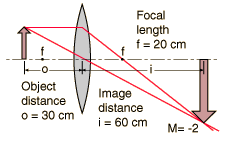
\includegraphics[scale=0.5]{img/thinLensEq.png}
        \caption{Model tenkej šošovky}
    \end{figure}

\end{frame}

\begin{frame}\frametitle{Rozdelenie aberácii}
    \begin{itemize}
        \item odchýlenie ľúčov od ohniskového bodu - Wikipedia
        \item \textbf{achromatické} \\
            \begin{itemize}
                \item rozostrenie
                \item deformácia 
            \end{itemize}
        \item \textbf{chromatické}
    \end{itemize}
    
\end{frame}


\begin{frame}\frametitle{Sférická aberácia}
    \begin{itemize}
        \item pararelné ľúče nie sú fokusované do jediného bodu\textit{optickej osi}
        \item \textbf{Dôsledok:} rozostretý obraz, \textit{circle of the least confusion}
        \item Riešienie: \textit{asférický tvar šošoviek}, korektory
    \end{itemize}

    \begin{columns}
    \column{0.5\textwidth}
    \begin{figure}
        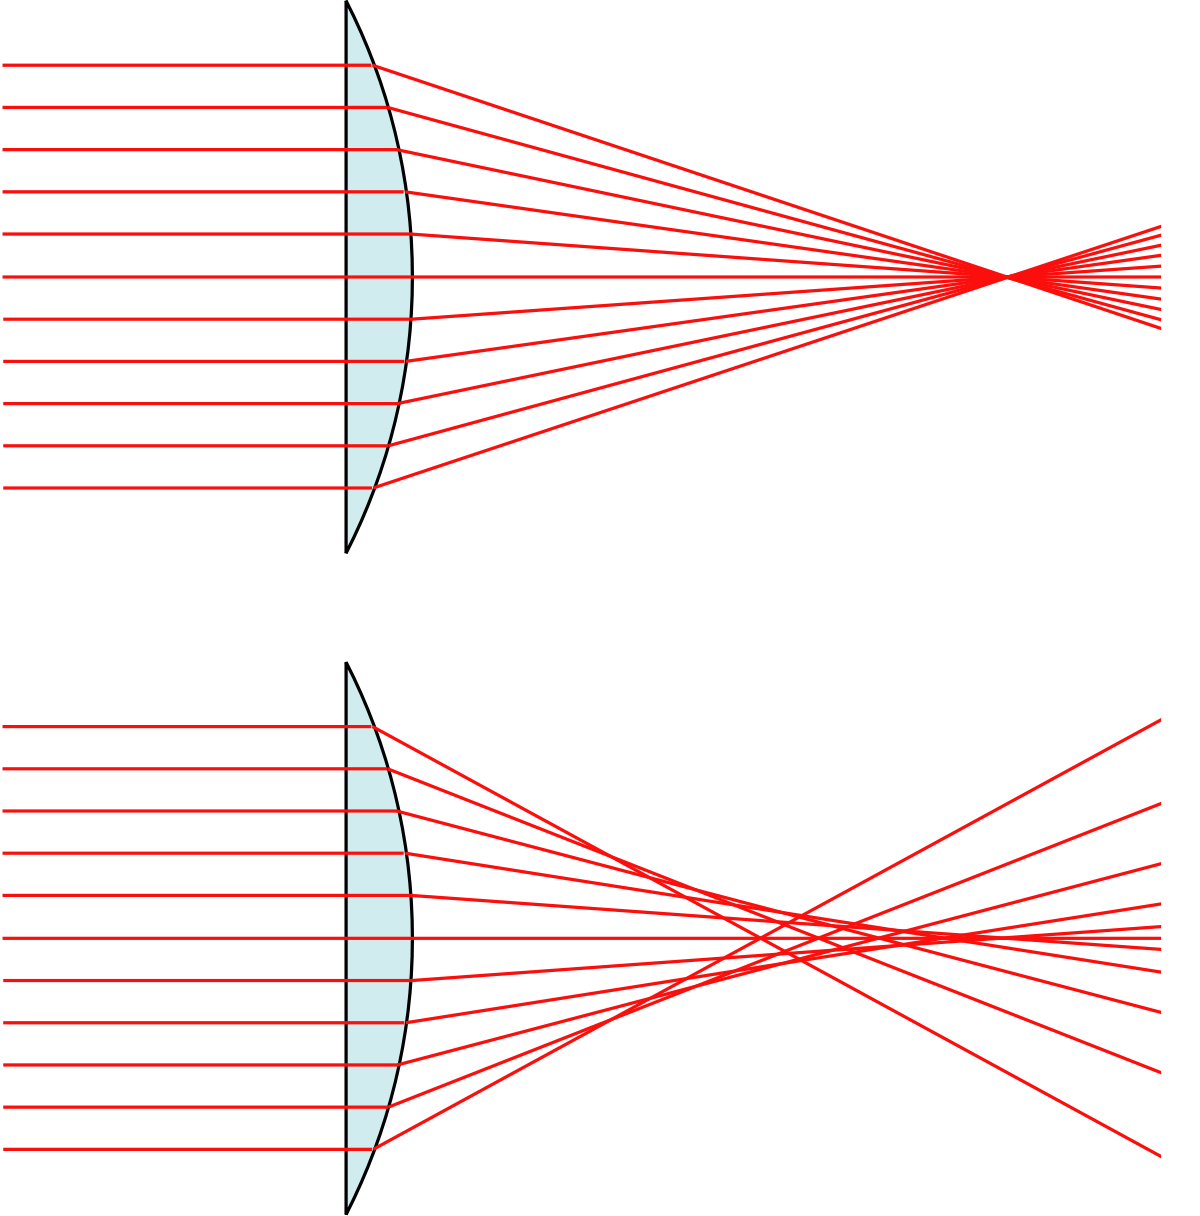
\includegraphics[scale=0.1]{img/sphericalAberrationWikipedia.png}
        \caption{Ideálna (hore) vs reálna šošovka (dole)}
    \end{figure}
    \column{0.5\textwidth}
    \begin{figure}
        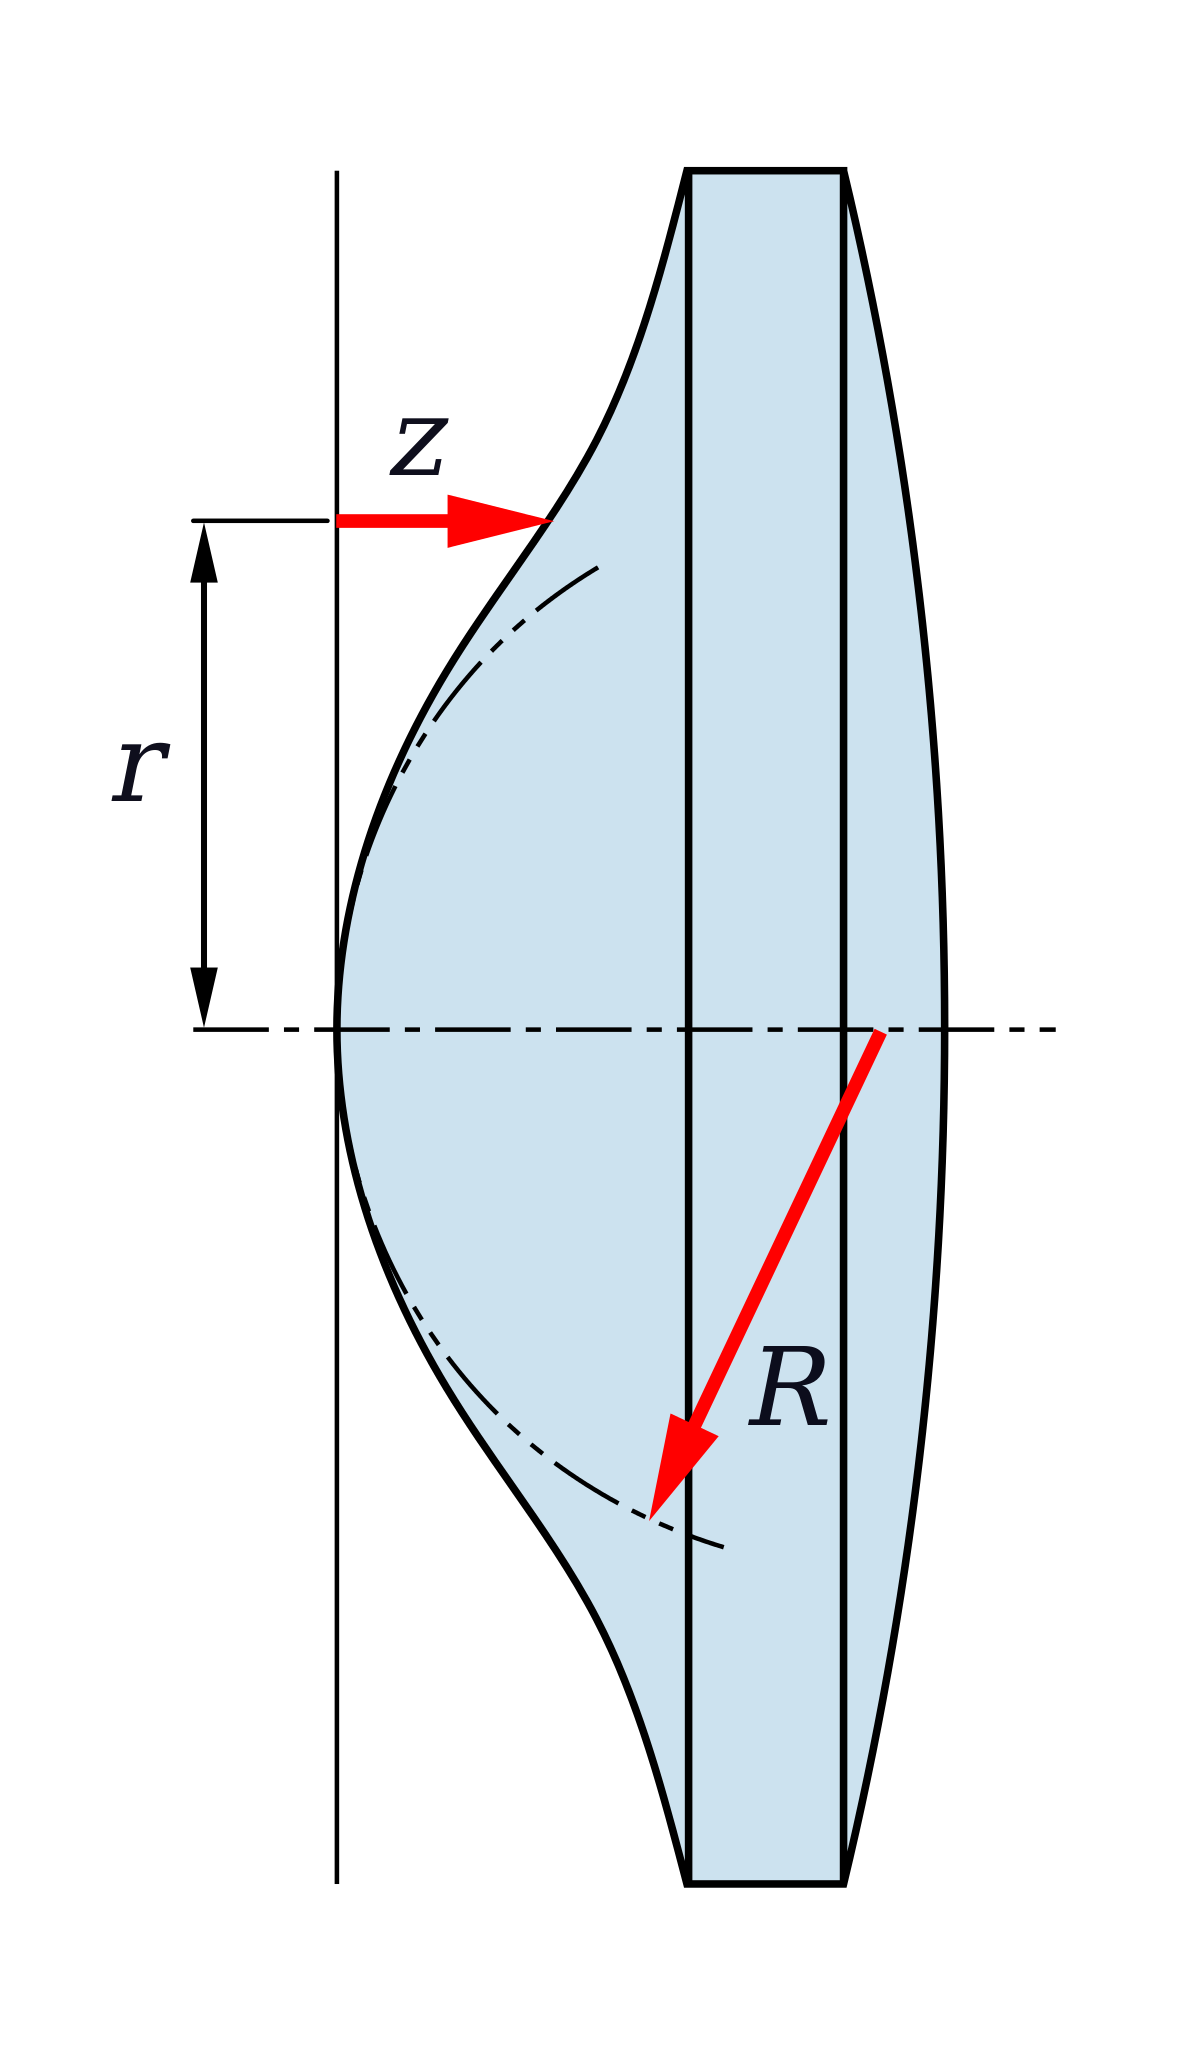
\includegraphics[scale=0.05]{img/asphericLen.png}
        \caption{Asférická šošovka}
    \end{figure}
    \end{columns}
\end{frame}

\begin{frame}\frametitle{Coma}
    \begin{itemize}
        \item rozmazanie bodových predmetov ležiacich mimo optickú osu 
        \item typickým prejavom je vznik chvosta (ang. \textit{coma}, česky \textit{ocas})
        \item \textbf{riešenie:} coma corrector, pre 1 vlnovú dĺžku aplanatické (asférické šošovky)
    \end{itemize}

    \begin{columns}
        \column{0.5\textwidth}
        \begin{figure}
            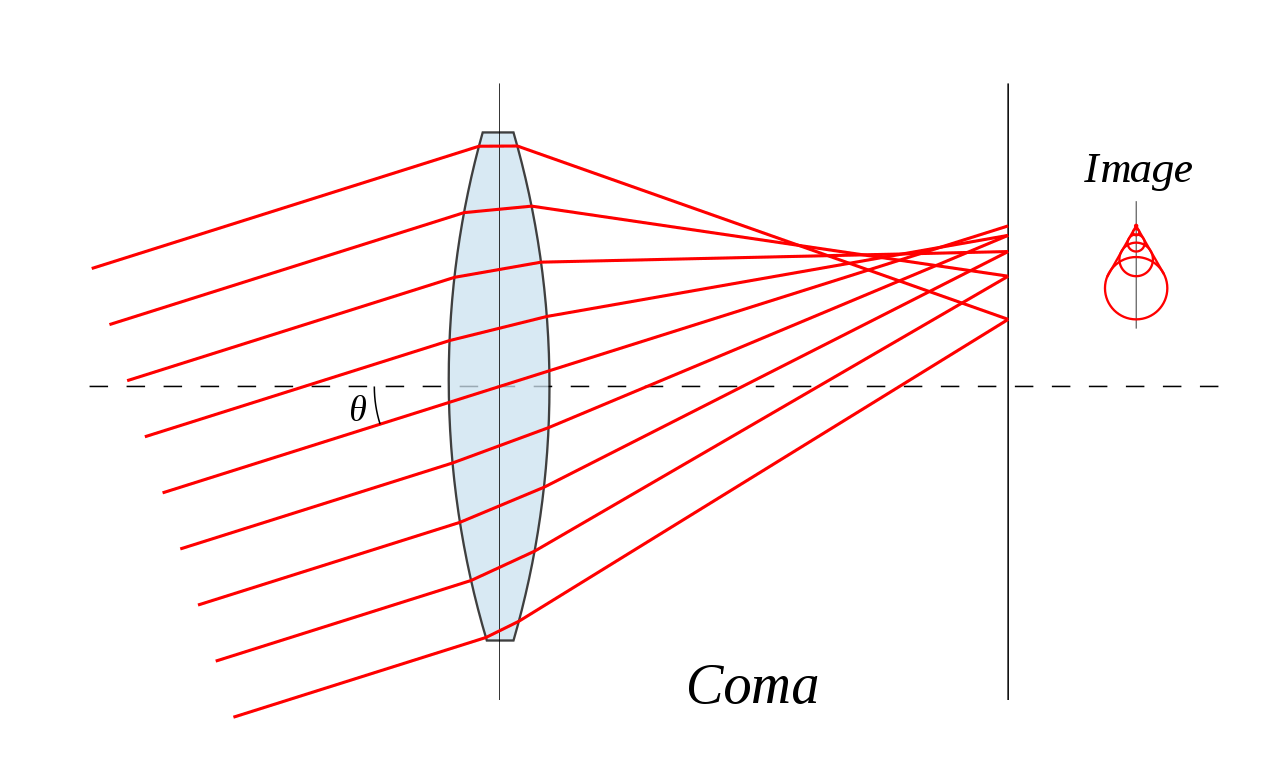
\includegraphics[scale=0.15]{img/coma.png}
        \end{figure}

        \column{0.5\textwidth}
        \begin{figure}
            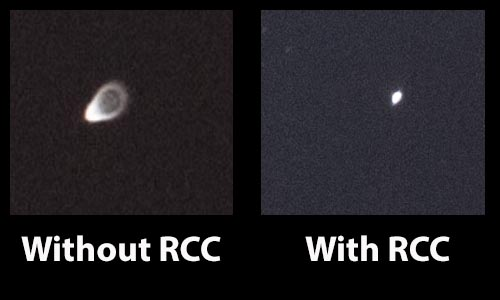
\includegraphics[scale=0.20]{img/coma.jpg}
            \caption{Baader Rowe Coma Corrector}
        \end{figure}
    \end{columns}
\end{frame}


\begin{frame}\frametitle{Petzvalovo zakrivenie pola}
    \begin{itemize}
        % http://www.wikiwand.com/en/Petzval_field_curvature
        \item lúče z naklonenej predmetovej roviny konvergujú na rovine 
        \item nemožno voliť obrazovú rovinu, nutno použiť zakrivenú rovinu
        \item nutno komenzovať: Kepler Space Center
    \end{itemize}
\end{frame}

\begin{frame}\frametitle{Astigmatizmus}
    \begin{itemize}
        \item lúče jednej roviny majú odlišné ohnisko od ľúčov roviny kolmej na ňu
    \end{itemize}
    \begin{figure}
        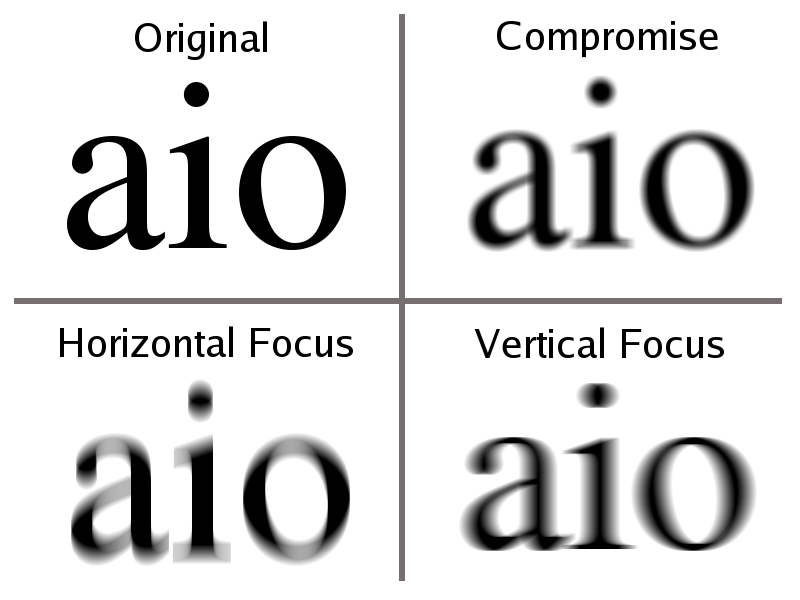
\includegraphics[scale=0.20]{img/astigmatism.png}
        \caption{Vizuálny astigmatizmus}
    \end{figure}
\end{frame}

\begin{frame}\frametitle{Chromaticka aberácia}
    \begin{itemize}
        \item index lomu je funkciou \textbf{vlnovej dĺžky}
        \item \textbf{Dôsledok:} rozostrenie podľa farebných zložiek
    \end{itemize}

    \begin{figure}
        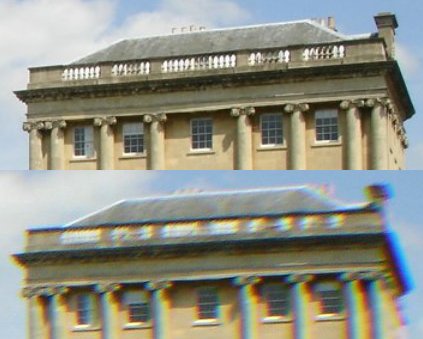
\includegraphics[scale=0.4]{img/chromaticAberrationWikipedia.jpg}
        \caption{lion!!}
    \end{figure}
    Riešienie: \textit{doublet}, SW korekcia 
\end{frame}

\begin{frame}\frametitle{Sférická aberácia}
    \begin{itemize}
        \item TODO
    \end{itemize}
\end{frame}

\bluepage{Ďakujem za vašu pozornosť / otázky}

\end{document}
